% Options for packages loaded elsewhere
\PassOptionsToPackage{unicode}{hyperref}
\PassOptionsToPackage{hyphens}{url}
\PassOptionsToPackage{dvipsnames,svgnames,x11names}{xcolor}
%
\documentclass[
  letterpaper,
  DIV=11,
  numbers=noendperiod]{scrreprt}

\usepackage{amsmath,amssymb}
\usepackage{iftex}
\ifPDFTeX
  \usepackage[T1]{fontenc}
  \usepackage[utf8]{inputenc}
  \usepackage{textcomp} % provide euro and other symbols
\else % if luatex or xetex
  \usepackage{unicode-math}
  \defaultfontfeatures{Scale=MatchLowercase}
  \defaultfontfeatures[\rmfamily]{Ligatures=TeX,Scale=1}
\fi
\usepackage{lmodern}
\ifPDFTeX\else  
    % xetex/luatex font selection
\fi
% Use upquote if available, for straight quotes in verbatim environments
\IfFileExists{upquote.sty}{\usepackage{upquote}}{}
\IfFileExists{microtype.sty}{% use microtype if available
  \usepackage[]{microtype}
  \UseMicrotypeSet[protrusion]{basicmath} % disable protrusion for tt fonts
}{}
\makeatletter
\@ifundefined{KOMAClassName}{% if non-KOMA class
  \IfFileExists{parskip.sty}{%
    \usepackage{parskip}
  }{% else
    \setlength{\parindent}{0pt}
    \setlength{\parskip}{6pt plus 2pt minus 1pt}}
}{% if KOMA class
  \KOMAoptions{parskip=half}}
\makeatother
\usepackage{xcolor}
\usepackage{svg}
\setlength{\emergencystretch}{3em} % prevent overfull lines
\setcounter{secnumdepth}{5}
% Make \paragraph and \subparagraph free-standing
\ifx\paragraph\undefined\else
  \let\oldparagraph\paragraph
  \renewcommand{\paragraph}[1]{\oldparagraph{#1}\mbox{}}
\fi
\ifx\subparagraph\undefined\else
  \let\oldsubparagraph\subparagraph
  \renewcommand{\subparagraph}[1]{\oldsubparagraph{#1}\mbox{}}
\fi

\usepackage{color}
\usepackage{fancyvrb}
\newcommand{\VerbBar}{|}
\newcommand{\VERB}{\Verb[commandchars=\\\{\}]}
\DefineVerbatimEnvironment{Highlighting}{Verbatim}{commandchars=\\\{\}}
% Add ',fontsize=\small' for more characters per line
\usepackage{framed}
\definecolor{shadecolor}{RGB}{241,243,245}
\newenvironment{Shaded}{\begin{snugshade}}{\end{snugshade}}
\newcommand{\AlertTok}[1]{\textcolor[rgb]{0.68,0.00,0.00}{#1}}
\newcommand{\AnnotationTok}[1]{\textcolor[rgb]{0.37,0.37,0.37}{#1}}
\newcommand{\AttributeTok}[1]{\textcolor[rgb]{0.40,0.45,0.13}{#1}}
\newcommand{\BaseNTok}[1]{\textcolor[rgb]{0.68,0.00,0.00}{#1}}
\newcommand{\BuiltInTok}[1]{\textcolor[rgb]{0.00,0.23,0.31}{#1}}
\newcommand{\CharTok}[1]{\textcolor[rgb]{0.13,0.47,0.30}{#1}}
\newcommand{\CommentTok}[1]{\textcolor[rgb]{0.37,0.37,0.37}{#1}}
\newcommand{\CommentVarTok}[1]{\textcolor[rgb]{0.37,0.37,0.37}{\textit{#1}}}
\newcommand{\ConstantTok}[1]{\textcolor[rgb]{0.56,0.35,0.01}{#1}}
\newcommand{\ControlFlowTok}[1]{\textcolor[rgb]{0.00,0.23,0.31}{#1}}
\newcommand{\DataTypeTok}[1]{\textcolor[rgb]{0.68,0.00,0.00}{#1}}
\newcommand{\DecValTok}[1]{\textcolor[rgb]{0.68,0.00,0.00}{#1}}
\newcommand{\DocumentationTok}[1]{\textcolor[rgb]{0.37,0.37,0.37}{\textit{#1}}}
\newcommand{\ErrorTok}[1]{\textcolor[rgb]{0.68,0.00,0.00}{#1}}
\newcommand{\ExtensionTok}[1]{\textcolor[rgb]{0.00,0.23,0.31}{#1}}
\newcommand{\FloatTok}[1]{\textcolor[rgb]{0.68,0.00,0.00}{#1}}
\newcommand{\FunctionTok}[1]{\textcolor[rgb]{0.28,0.35,0.67}{#1}}
\newcommand{\ImportTok}[1]{\textcolor[rgb]{0.00,0.46,0.62}{#1}}
\newcommand{\InformationTok}[1]{\textcolor[rgb]{0.37,0.37,0.37}{#1}}
\newcommand{\KeywordTok}[1]{\textcolor[rgb]{0.00,0.23,0.31}{#1}}
\newcommand{\NormalTok}[1]{\textcolor[rgb]{0.00,0.23,0.31}{#1}}
\newcommand{\OperatorTok}[1]{\textcolor[rgb]{0.37,0.37,0.37}{#1}}
\newcommand{\OtherTok}[1]{\textcolor[rgb]{0.00,0.23,0.31}{#1}}
\newcommand{\PreprocessorTok}[1]{\textcolor[rgb]{0.68,0.00,0.00}{#1}}
\newcommand{\RegionMarkerTok}[1]{\textcolor[rgb]{0.00,0.23,0.31}{#1}}
\newcommand{\SpecialCharTok}[1]{\textcolor[rgb]{0.37,0.37,0.37}{#1}}
\newcommand{\SpecialStringTok}[1]{\textcolor[rgb]{0.13,0.47,0.30}{#1}}
\newcommand{\StringTok}[1]{\textcolor[rgb]{0.13,0.47,0.30}{#1}}
\newcommand{\VariableTok}[1]{\textcolor[rgb]{0.07,0.07,0.07}{#1}}
\newcommand{\VerbatimStringTok}[1]{\textcolor[rgb]{0.13,0.47,0.30}{#1}}
\newcommand{\WarningTok}[1]{\textcolor[rgb]{0.37,0.37,0.37}{\textit{#1}}}

\providecommand{\tightlist}{%
  \setlength{\itemsep}{0pt}\setlength{\parskip}{0pt}}\usepackage{longtable,booktabs,array}
\usepackage{calc} % for calculating minipage widths
% Correct order of tables after \paragraph or \subparagraph
\usepackage{etoolbox}
\makeatletter
\patchcmd\longtable{\par}{\if@noskipsec\mbox{}\fi\par}{}{}
\makeatother
% Allow footnotes in longtable head/foot
\IfFileExists{footnotehyper.sty}{\usepackage{footnotehyper}}{\usepackage{footnote}}
\makesavenoteenv{longtable}
\usepackage{graphicx}
\makeatletter
\def\maxwidth{\ifdim\Gin@nat@width>\linewidth\linewidth\else\Gin@nat@width\fi}
\def\maxheight{\ifdim\Gin@nat@height>\textheight\textheight\else\Gin@nat@height\fi}
\makeatother
% Scale images if necessary, so that they will not overflow the page
% margins by default, and it is still possible to overwrite the defaults
% using explicit options in \includegraphics[width, height, ...]{}
\setkeys{Gin}{width=\maxwidth,height=\maxheight,keepaspectratio}
% Set default figure placement to htbp
\makeatletter
\def\fps@figure{htbp}
\makeatother

\KOMAoption{captions}{tableheading}
\makeatletter
\makeatother
\makeatletter
\@ifpackageloaded{bookmark}{}{\usepackage{bookmark}}
\makeatother
\makeatletter
\@ifpackageloaded{caption}{}{\usepackage{caption}}
\AtBeginDocument{%
\ifdefined\contentsname
  \renewcommand*\contentsname{Table of contents}
\else
  \newcommand\contentsname{Table of contents}
\fi
\ifdefined\listfigurename
  \renewcommand*\listfigurename{List of Figures}
\else
  \newcommand\listfigurename{List of Figures}
\fi
\ifdefined\listtablename
  \renewcommand*\listtablename{List of Tables}
\else
  \newcommand\listtablename{List of Tables}
\fi
\ifdefined\figurename
  \renewcommand*\figurename{Figure}
\else
  \newcommand\figurename{Figure}
\fi
\ifdefined\tablename
  \renewcommand*\tablename{Table}
\else
  \newcommand\tablename{Table}
\fi
}
\@ifpackageloaded{float}{}{\usepackage{float}}
\floatstyle{ruled}
\@ifundefined{c@chapter}{\newfloat{codelisting}{h}{lop}}{\newfloat{codelisting}{h}{lop}[chapter]}
\floatname{codelisting}{Listing}
\newcommand*\listoflistings{\listof{codelisting}{List of Listings}}
\makeatother
\makeatletter
\@ifpackageloaded{caption}{}{\usepackage{caption}}
\@ifpackageloaded{subcaption}{}{\usepackage{subcaption}}
\makeatother
\makeatletter
\@ifpackageloaded{tcolorbox}{}{\usepackage[skins,breakable]{tcolorbox}}
\makeatother
\makeatletter
\@ifundefined{shadecolor}{\definecolor{shadecolor}{rgb}{.97, .97, .97}}
\makeatother
\makeatletter
\makeatother
\makeatletter
\makeatother
\ifLuaTeX
  \usepackage{selnolig}  % disable illegal ligatures
\fi
\IfFileExists{bookmark.sty}{\usepackage{bookmark}}{\usepackage{hyperref}}
\IfFileExists{xurl.sty}{\usepackage{xurl}}{} % add URL line breaks if available
\urlstyle{same} % disable monospaced font for URLs
\hypersetup{
  pdftitle={{[}STUDENT{]} Progress Journal},
  colorlinks=true,
  linkcolor={blue},
  filecolor={Maroon},
  citecolor={Blue},
  urlcolor={Blue},
  pdfcreator={LaTeX via pandoc}}

\title{{[}STUDENT{]} Progress Journal}
\author{}
\date{}

\begin{document}
\maketitle
\ifdefined\Shaded\renewenvironment{Shaded}{\begin{tcolorbox}[boxrule=0pt, sharp corners, breakable, borderline west={3pt}{0pt}{shadecolor}, frame hidden, enhanced, interior hidden]}{\end{tcolorbox}}\fi

\renewcommand*\contentsname{Table of contents}
{
\hypersetup{linkcolor=}
\setcounter{tocdepth}{2}
\tableofcontents
}
\bookmarksetup{startatroot}

\hypertarget{introduction}{%
\chapter*{Introduction}\label{introduction}}
\addcontentsline{toc}{chapter}{Introduction}

\markboth{Introduction}{Introduction}

This progress journal covers {[}STUDENT NAME SURNAME / PROJECT GROUP
NAME{]}'s work during their term at
\href{https://mef-bda503.github.io/fall22/}{BDA 503 Fall 2022}.

Each section is an assignment or an individual work.

\bookmarksetup{startatroot}

\hypertarget{assignment-1}{%
\chapter{Assignment 1}\label{assignment-1}}

\hypertarget{about-me}{%
\section{About Me}\label{about-me}}

I'm \textbf{Gözde Uğur}. I've been working as Senior Data Analyst at
Trendyol for almost 2 years. Since graduating from university, I have
worked in various data analyst roles where I mainly used SQL. I want to
make sophisticated analyzes and visualizations of data with what I
learned in this program. You can check
\href{https://www.linkedin.com/in/gozde-ugur-000/}{My Linkedin Page} for
further info.

\hypertarget{bridging-the-gap-between-sql-and-r}{%
\section{Bridging the Gap between SQL and
R}\label{bridging-the-gap-between-sql-and-r}}

The reason I chose this video called
\href{https://www.youtube.com/watch?v=JwP5KdWSgqE\&list=PL9HYL-VRX0oTOK4cpbCbRk15K2roEgzVW\&t=1094s}{\emph{Bridging
the Gap between SQL and R}} was that I was curious about ways to use
SQL, which I use frequently in daily life, in R. In this video, I
learned an R package, tidyquery, with which I can run SQL Queries
directly.

\hypertarget{dataset}{%
\section{Dataset}\label{dataset}}

\hypertarget{amazon-products-dataset-2023}{%
\subsection{Amazon Products Dataset
2023}\label{amazon-products-dataset-2023}}

\begin{Shaded}
\begin{Highlighting}[]
\FunctionTok{library}\NormalTok{(dplyr)}
\end{Highlighting}
\end{Shaded}

\begin{verbatim}

Attaching package: 'dplyr'
\end{verbatim}

\begin{verbatim}
The following objects are masked from 'package:stats':

    filter, lag
\end{verbatim}

\begin{verbatim}
The following objects are masked from 'package:base':

    intersect, setdiff, setequal, union
\end{verbatim}

\begin{Shaded}
\begin{Highlighting}[]
\CommentTok{\# Using read.csv()}
\NormalTok{myData }\OtherTok{=} \FunctionTok{read.csv}\NormalTok{(}\StringTok{"/Users/gozde.ugur/Downloads/archive (3)/amazon\_products.csv"}\NormalTok{) }
\NormalTok{en\_cok\_satanlar }\OtherTok{\textless{}{-}}\NormalTok{ myData }\SpecialCharTok{\%\textgreater{}\%} 
  \FunctionTok{arrange}\NormalTok{(}\FunctionTok{desc}\NormalTok{(boughtInLastMonth)) }\SpecialCharTok{\%\textgreater{}\%}  \CommentTok{\# satisadedi sütununa göre azalan sırada sırala}
  \FunctionTok{head}\NormalTok{(}\DecValTok{5}\NormalTok{)  }\CommentTok{\# İlk 5 kaydı getirilk\_5\_kayit \textless{}{-} head(myData, 5)}
\CommentTok{\# Show only selected columns}
\NormalTok{secilen\_sutunlar }\OtherTok{\textless{}{-}}\NormalTok{ en\_cok\_satanlar[, }\FunctionTok{c}\NormalTok{(}\StringTok{"title"}\NormalTok{,}\StringTok{"stars"}\NormalTok{, }\StringTok{"price"}\NormalTok{ ,}\StringTok{"boughtInLastMonth"}\NormalTok{)]}
\FunctionTok{print}\NormalTok{(secilen\_sutunlar)}
\end{Highlighting}
\end{Shaded}

\begin{verbatim}
                                                                                                                                                                            title
1                                                                                                        Bounty Quick Size Paper Towels, White, 8 Family Rolls = 20 Regular Rolls
2                                            Amazon Brand - Presto! Flex-a-Size Paper Towels, 158 Sheet Huge Roll, 12 Rolls (2 Packs of 6), Equivalent to 38 Regular Rolls, White
3                                                                                                             Stardrops - The Pink Stuff - The Miracle All Purpose Cleaning Paste
4                                                                              Amazon Basics 2-Ply Paper Towels, Flex-Sheets, 150 Sheets per Roll, 12 Rolls (2 Packs of 6), White
5 Hismile v34 Colour Corrector, Tooth Stain Removal, Teeth Whitening Booster, Purple Toothpaste, Colour Correcting, Hismile V34, Hismile Colour Corrector, Tooth Colour Corrector
  stars price boughtInLastMonth
1   4.8 24.42            100000
2   4.7 28.28            100000
3   4.4  4.99            100000
4   4.2 22.86            100000
5   3.4 20.69            100000
\end{verbatim}

Since I work in the e-commerce industry,
\href{https://www.kaggle.com/datasets/asaniczka/amazon-products-dataset-2023-1-4m-products}{\textbf{Amazon
Products Dataset 2023}} attracted my attention. Reasons why I find this
dataset useful for out course:

1. We may have the opportunity to get more insight about the trends and
behaviors in the e-commerce industry, where we are usually on the
customer side.

2. This dataset allows us to work with different data types such as
boolean, integer, float and character.

3. This dataset contains 1.4M records. Although we work with much larger
datasets in real business life, working with this dataset can also be a
good opportunity to learn and overcome the difficulties of large
datasets.

\hypertarget{r-posts-relevant-to-my-interests}{%
\section{R posts relevant to my
interests}\label{r-posts-relevant-to-my-interests}}

\hypertarget{r-histogram}{%
\section{R Histogram}\label{r-histogram}}

A histogram is like a bar chart as it uses bars of varying height to
represent data distribution. However, in a histogram values are grouped
into consecutive intervals called bins. In a Histogram, continuous
values are grouped and displayed in these bins whose size can be varied.

\textbf{Example:}~

\begin{Shaded}
\begin{Highlighting}[]
\CommentTok{\# Histogram for Maximum Daily Temperature }
\FunctionTok{data}\NormalTok{(airquality) }

\FunctionTok{hist}\NormalTok{(airquality}\SpecialCharTok{$}\NormalTok{Temp, }\AttributeTok{main =}\StringTok{"La Guardia Airport\textquotesingle{}s\textbackslash{} }
\StringTok{Maximum Temperature(Daily)"}\NormalTok{, }
    \AttributeTok{xlab =}\StringTok{"Temperature(Fahrenheit)"}\NormalTok{, }
    \AttributeTok{xlim =} \FunctionTok{c}\NormalTok{(}\DecValTok{50}\NormalTok{, }\DecValTok{125}\NormalTok{), }\AttributeTok{col =}\StringTok{"yellow"}\NormalTok{, }
    \AttributeTok{freq =} \ConstantTok{TRUE}\NormalTok{) }
\end{Highlighting}
\end{Shaded}

\begin{figure}[H]

{\centering 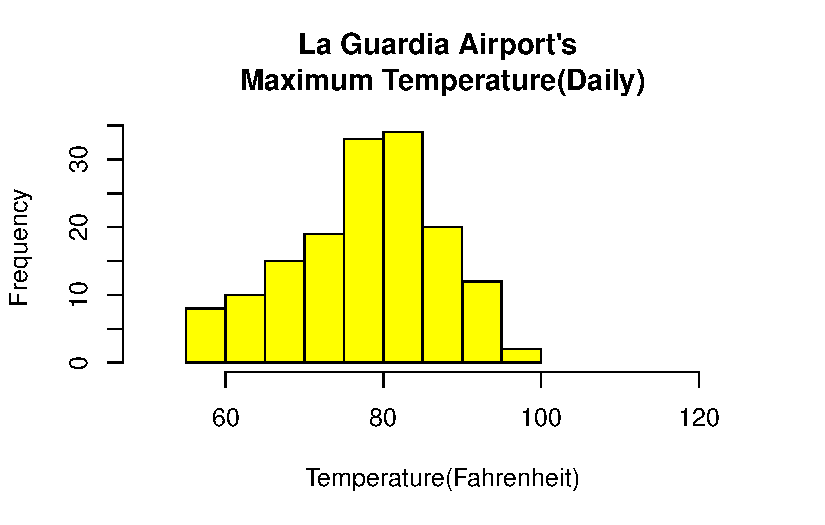
\includegraphics{assignment1_files/figure-pdf/unnamed-chunk-2-1.pdf}

}

\end{figure}

\hypertarget{hypothesis-testing-in-r-programming}{%
\section{Hypothesis Testing in R
Programming}\label{hypothesis-testing-in-r-programming}}

hypothesis is made by the researchers about the data collected for any
experiment or data set. A hypothesis is an assumption made by the
researchers that are not mandatory true. In simple words, a hypothesis
is a decision taken by the researchers based on the data of the
population collected.
\href{https://www.geeksforgeeks.org/understanding-hypothesis-testing/}{\textbf{Hypothesis
Testing}} in
\href{https://www.geeksforgeeks.org/introduction-to-r-programming-language/}{\textbf{R
Programming}} is a process of testing the hypothesis made by the
researcher or to validate the hypothesis. To perform hypothesis testing,
a random sample of data from the population is taken and testing is
performed. Based on the results of the testing, the hypothesis is either
selected or rejected. This concept is known as \textbf{Statistical
Inference}. In this article, we'll discuss the four-step process of
hypothesis testing, One sample T-Testing, Two-sample T-Testing,
Directional Hypothesis, one
sample~\includesvg{index_files/mediabag/quicklatex.com-be5d4.svg}-test,
two
samples~\includesvg{index_files/mediabag/quicklatex.com-be5d4.svg}-test
and correlation test in R programming.

\hypertarget{one-sample-t-testing}{%
\subsubsection{One Sample T-Testing}\label{one-sample-t-testing}}

One sample T-Testing approach collects a huge amount of data and tests
it on random samples. To perform T-Test in R, normally distributed data
is required. This test is used to test the mean of the sample with the
population. For example, the height of persons living in an area is
different or identical to other persons living in other areas.

\begin{quote}
\textbf{Syntax:} t.test(x, mu) \textbf{Parameters:} \textbf{x:}
represents numeric vector of data \textbf{mu:} represents true value of
the mean
\end{quote}

To know about more optional parameters of \textbf{t.test()}, try the
below command:

\begin{verbatim}
help("t.test")
\end{verbatim}

\textbf{Example:}~

\begin{Shaded}
\begin{Highlighting}[]
\CommentTok{\# Defining sample vector}
\NormalTok{x }\OtherTok{\textless{}{-}} \FunctionTok{rnorm}\NormalTok{(}\DecValTok{100}\NormalTok{)}

\CommentTok{\# One Sample T{-}Test}
\FunctionTok{t.test}\NormalTok{(x, }\AttributeTok{mu =} \DecValTok{5}\NormalTok{)}
\end{Highlighting}
\end{Shaded}

\begin{verbatim}

    One Sample t-test

data:  x
t = -52.532, df = 99, p-value < 2.2e-16
alternative hypothesis: true mean is not equal to 5
95 percent confidence interval:
 -0.07730987  0.29228311
sample estimates:
mean of x 
0.1074866 
\end{verbatim}

\hypertarget{reading-a-.csv-file-in-r}{%
\section{Reading a .csv File in R}\label{reading-a-.csv-file-in-r}}

\textbf{read.csv()}: read.csv() is used for reading ``comma separated
value'' files (``.csv''). In this also the data will be imported as a
data frame.

\begin{quote}
\textbf{Syntax:} read.csv(file, header = TRUE, sep = ``,'', dec = ``.'',
\ldots)

\textbf{Parameters:}

\begin{itemize}
\item
  file: the path to the file containing the data to be imported into R.
\item
  header: logical value. If TRUE, read.csv() assumes that your file has
  a header row, so row 1 is the name of each column. If that's not the
  case, you can add the argument header = FALSE.
\item
  sep: the field separator character
\item
  dec: the character used in the file for decimal points.

\begin{Shaded}
\begin{Highlighting}[]
\FunctionTok{library}\NormalTok{(dplyr)}
\CommentTok{\# Using read.csv()}
\NormalTok{myData }\OtherTok{=} \FunctionTok{read.csv}\NormalTok{(}\StringTok{"/Users/gozde.ugur/Downloads/movies.csv"}\NormalTok{) }
\CommentTok{\# Show only first 5 record}
\NormalTok{comedy\_filmler }\OtherTok{\textless{}{-}}\NormalTok{ myData }\SpecialCharTok{\%\textgreater{}\%} \FunctionTok{filter}\NormalTok{(Genre }\SpecialCharTok{==} \StringTok{"Comedy"}\NormalTok{)}

\NormalTok{ilk\_5\_kayit }\OtherTok{\textless{}{-}} \FunctionTok{head}\NormalTok{(comedy\_filmler, }\DecValTok{5}\NormalTok{)}
\CommentTok{\# Show only selected columns}
\NormalTok{secilen\_sutunlar }\OtherTok{\textless{}{-}}\NormalTok{ ilk\_5\_kayit[, }\FunctionTok{c}\NormalTok{(}\StringTok{"Film"}\NormalTok{, }\StringTok{"Genre"}\NormalTok{, }\StringTok{"Year"}\NormalTok{)]}
\FunctionTok{print}\NormalTok{(secilen\_sutunlar)}
\end{Highlighting}
\end{Shaded}

\begin{verbatim}
                                Film  Genre Year
1                    Youth in Revolt Comedy 2010
2 You Will Meet a Tall Dark Stranger Comedy 2010
3                       When in Rome Comedy 2010
4              What Happens in Vegas Comedy 2008
5                    Valentine's Day Comedy 2010
\end{verbatim}
\end{itemize}
\end{quote}

\bookmarksetup{startatroot}

\hypertarget{inclass1}{%
\chapter{inclass1}\label{inclass1}}

\hypertarget{amazon-products-dataset-2023-1}{%
\subsection{Amazon Products Dataset
2023}\label{amazon-products-dataset-2023-1}}

\begin{Shaded}
\begin{Highlighting}[]
\FunctionTok{library}\NormalTok{(dplyr)}
\end{Highlighting}
\end{Shaded}

\begin{verbatim}

Attaching package: 'dplyr'
\end{verbatim}

\begin{verbatim}
The following objects are masked from 'package:stats':

    filter, lag
\end{verbatim}

\begin{verbatim}
The following objects are masked from 'package:base':

    intersect, setdiff, setequal, union
\end{verbatim}

\begin{Shaded}
\begin{Highlighting}[]
\CommentTok{\# Using read.csv()}
\NormalTok{myData }\OtherTok{=} \FunctionTok{read.csv}\NormalTok{(}\StringTok{"/Users/gozde.ugur/Downloads/archive (3)/amazon\_products.csv"}\NormalTok{) }
\NormalTok{en\_cok\_satanlar }\OtherTok{\textless{}{-}}\NormalTok{ myData }\SpecialCharTok{\%\textgreater{}\%} 
  \FunctionTok{arrange}\NormalTok{(}\FunctionTok{desc}\NormalTok{(boughtInLastMonth)) }\SpecialCharTok{\%\textgreater{}\%}  \CommentTok{\# satisadedi sütununa göre azalan sırada sırala}
  \FunctionTok{head}\NormalTok{(}\DecValTok{5}\NormalTok{)  }\CommentTok{\# İlk 5 kaydı getirilk\_5\_kayit }
\CommentTok{\# Show only selected columns}
\NormalTok{top\_5 }\OtherTok{\textless{}{-}}\NormalTok{ en\_cok\_satanlar[, }\FunctionTok{c}\NormalTok{(}\StringTok{"title"}\NormalTok{,}\StringTok{"stars"}\NormalTok{, }\StringTok{"price"}\NormalTok{ ,}\StringTok{"boughtInLastMonth"}\NormalTok{)]}
\FunctionTok{print}\NormalTok{(top\_5)}
\end{Highlighting}
\end{Shaded}

\begin{verbatim}
                                                                                                                                                                            title
1                                                                                                        Bounty Quick Size Paper Towels, White, 8 Family Rolls = 20 Regular Rolls
2                                            Amazon Brand - Presto! Flex-a-Size Paper Towels, 158 Sheet Huge Roll, 12 Rolls (2 Packs of 6), Equivalent to 38 Regular Rolls, White
3                                                                                                             Stardrops - The Pink Stuff - The Miracle All Purpose Cleaning Paste
4                                                                              Amazon Basics 2-Ply Paper Towels, Flex-Sheets, 150 Sheets per Roll, 12 Rolls (2 Packs of 6), White
5 Hismile v34 Colour Corrector, Tooth Stain Removal, Teeth Whitening Booster, Purple Toothpaste, Colour Correcting, Hismile V34, Hismile Colour Corrector, Tooth Colour Corrector
  stars price boughtInLastMonth
1   4.8 24.42            100000
2   4.7 28.28            100000
3   4.4  4.99            100000
4   4.2 22.86            100000
5   3.4 20.69            100000
\end{verbatim}

\begin{Shaded}
\begin{Highlighting}[]
\CommentTok{\#kategori bazında grupla, satışları topla}
\NormalTok{category\_sales }\OtherTok{\textless{}{-}}\NormalTok{ myData }\SpecialCharTok{\%\textgreater{}\%} 
                  \FunctionTok{group\_by}\NormalTok{(category\_id) }\SpecialCharTok{\%\textgreater{}\%}
                  \FunctionTok{summarise}\NormalTok{(}\AttributeTok{category\_sale=}\FunctionTok{sum}\NormalTok{(boughtInLastMonth)) }\SpecialCharTok{\%\textgreater{}\%}
                  \FunctionTok{ungroup}\NormalTok{()}


\FunctionTok{print}\NormalTok{(category\_sales)}
\end{Highlighting}
\end{Shaded}

\begin{verbatim}
# A tibble: 248 x 2
   category_id category_sale
         <int>         <int>
 1           1       1099750
 2           2         67400
 3           3        262100
 4           4        145050
 5           5        500500
 6           6       1509950
 7           7         46650
 8           8        128550
 9           9        197550
10          10       2092300
# i 238 more rows
\end{verbatim}



\end{document}
